%!TEX root = ../../thesis.tex

\section{Word properties}
\label{chapter:limitations:wordlproperties}


\question{How the world properties (symmetries, size, \ldots) affect the learning properties?}

xp with a grid world versus a pick and place with many wall and see that random becomes bad

refer to expeirmne in 5x5 grid world in section planning for 2d data and 90-100 data qualtities

refer to expeirmne with pick and place in section lfui and random planning (even if dtaset the same after 100 step no confidence)

50 run each method each world
90-95 percent datasets


\begin{figure}[!ht]
\centering
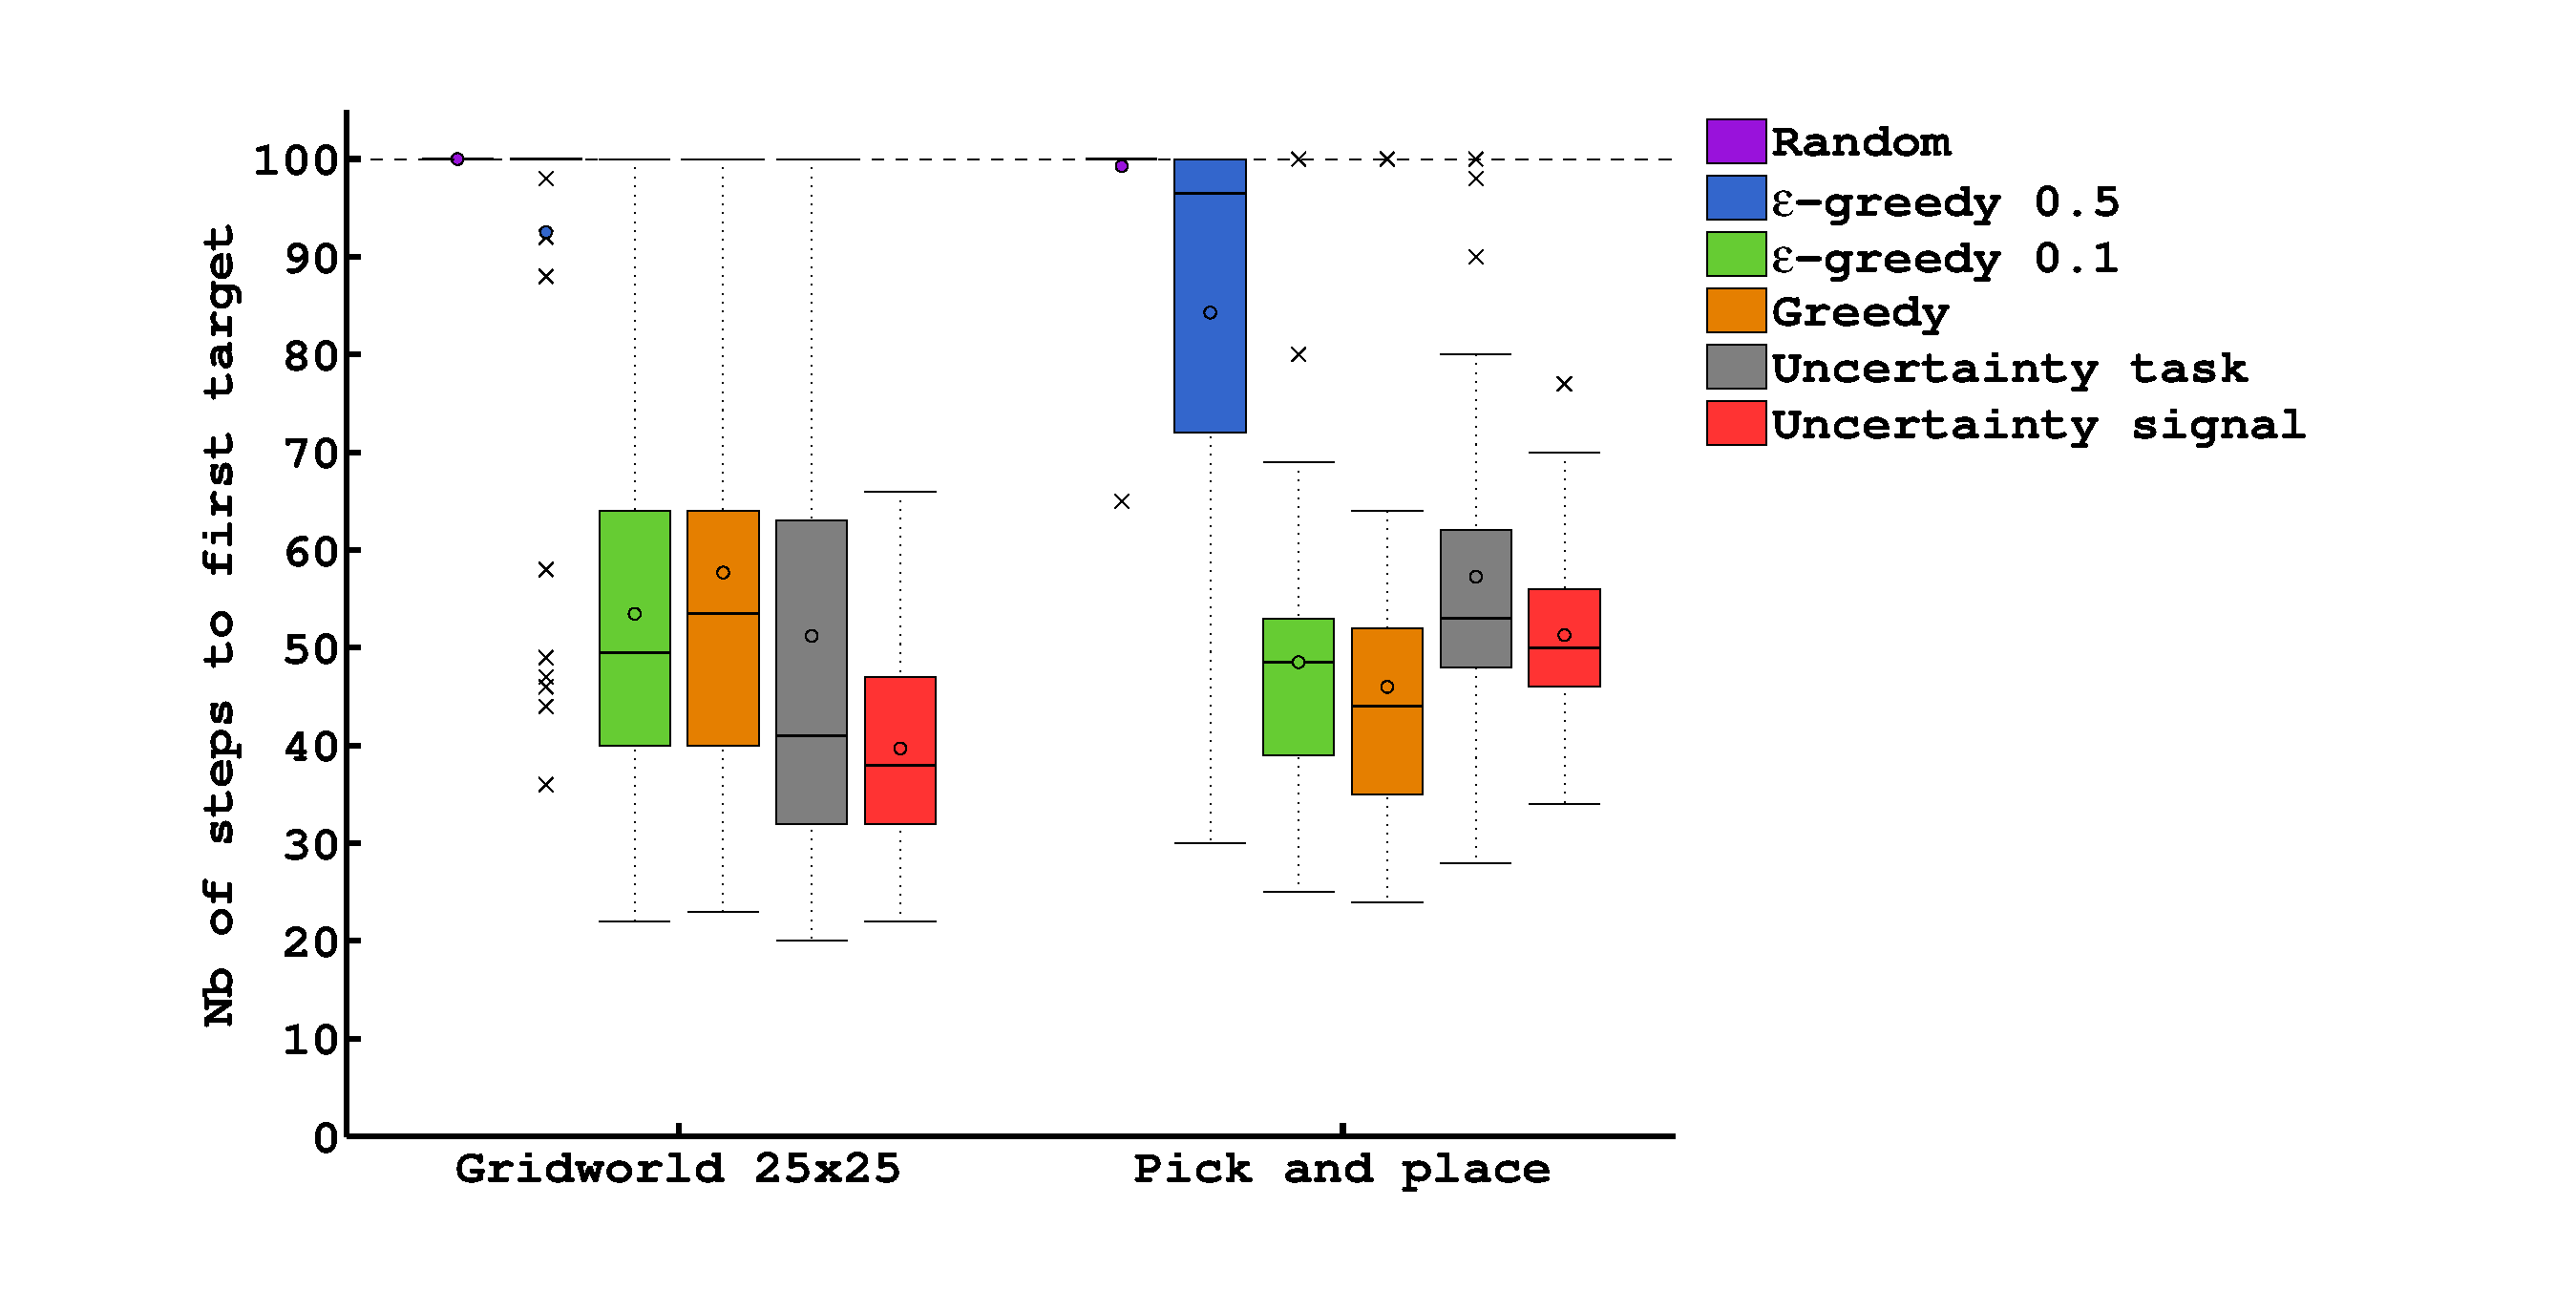
\includegraphics[width=\legendsidesize\columnwidth]{\imgpath/world_properties/firstreach.eps}
\caption{Number of steps to reach first target state with confidence.}
\label{fig:wordlpropertiestimefirst}
\end{figure} 

% nWrongFirstTarget =

%      0     0
%      0     1
%      0     2
%      1     2
%      0     1
%      0     2

\begin{figure}[!ht]
\centering
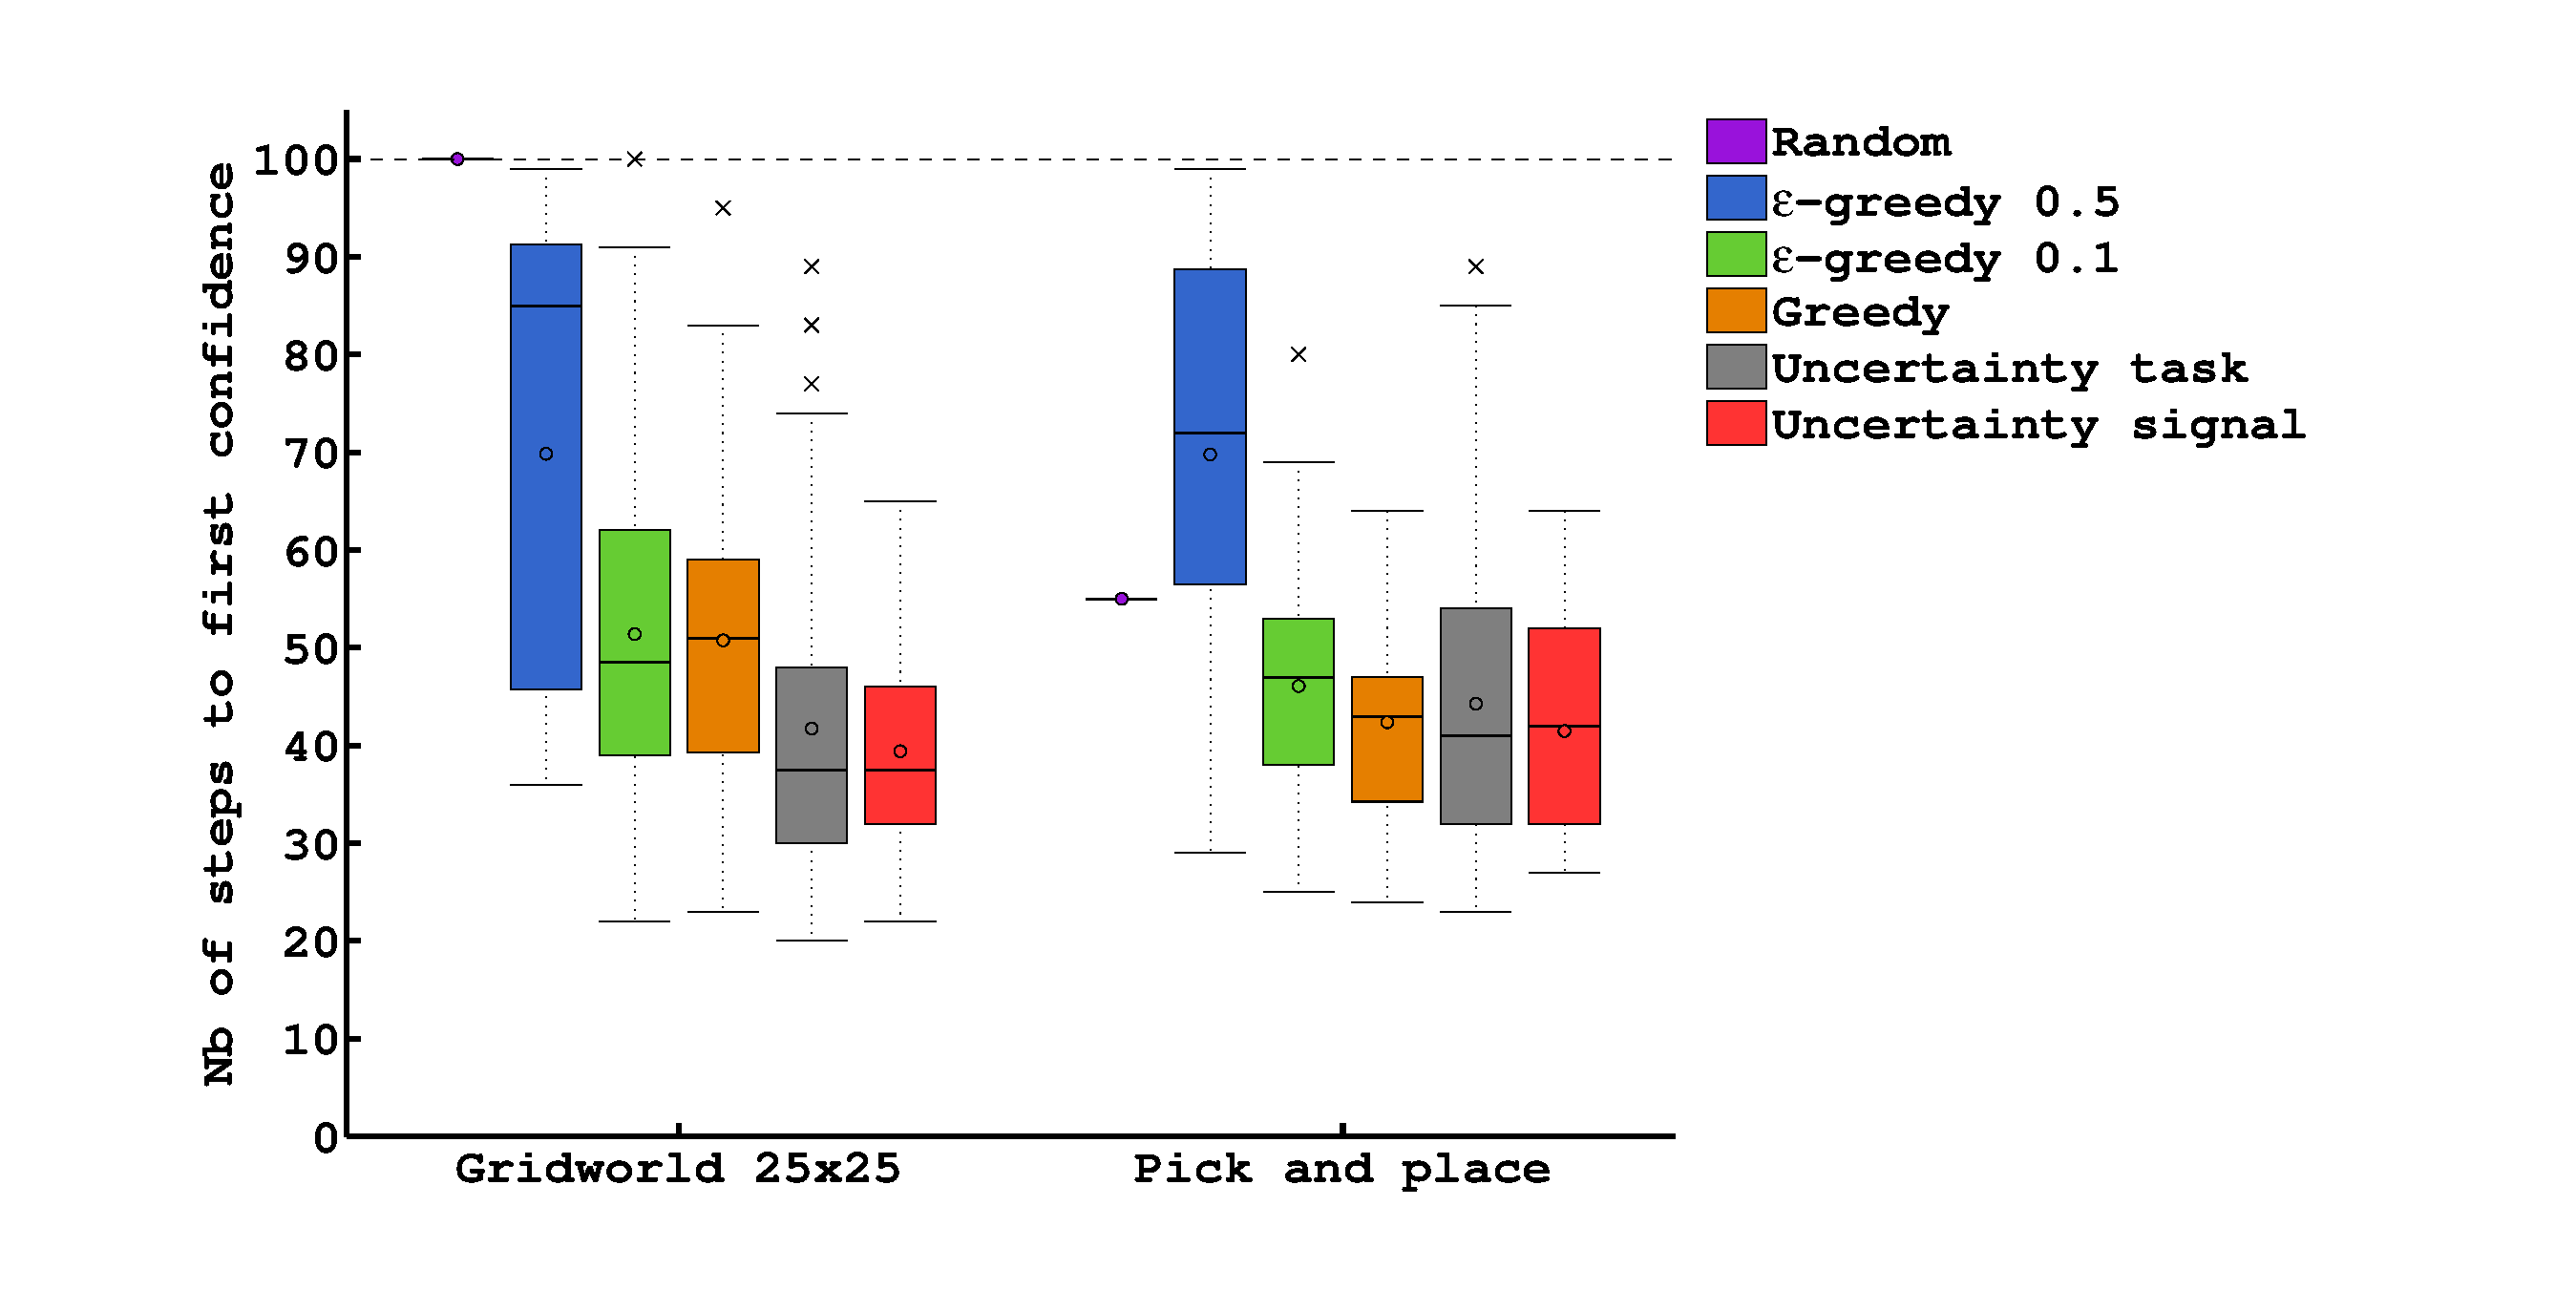
\includegraphics[width=\legendsidesize\columnwidth]{\imgpath/world_properties/firstconfident.eps}
\caption{Number of steps to reach confidence level for the first target.}
\label{fig:wordlpropertiesconfidencefirst}
\end{figure} 

\begin{figure}[!ht]
\centering
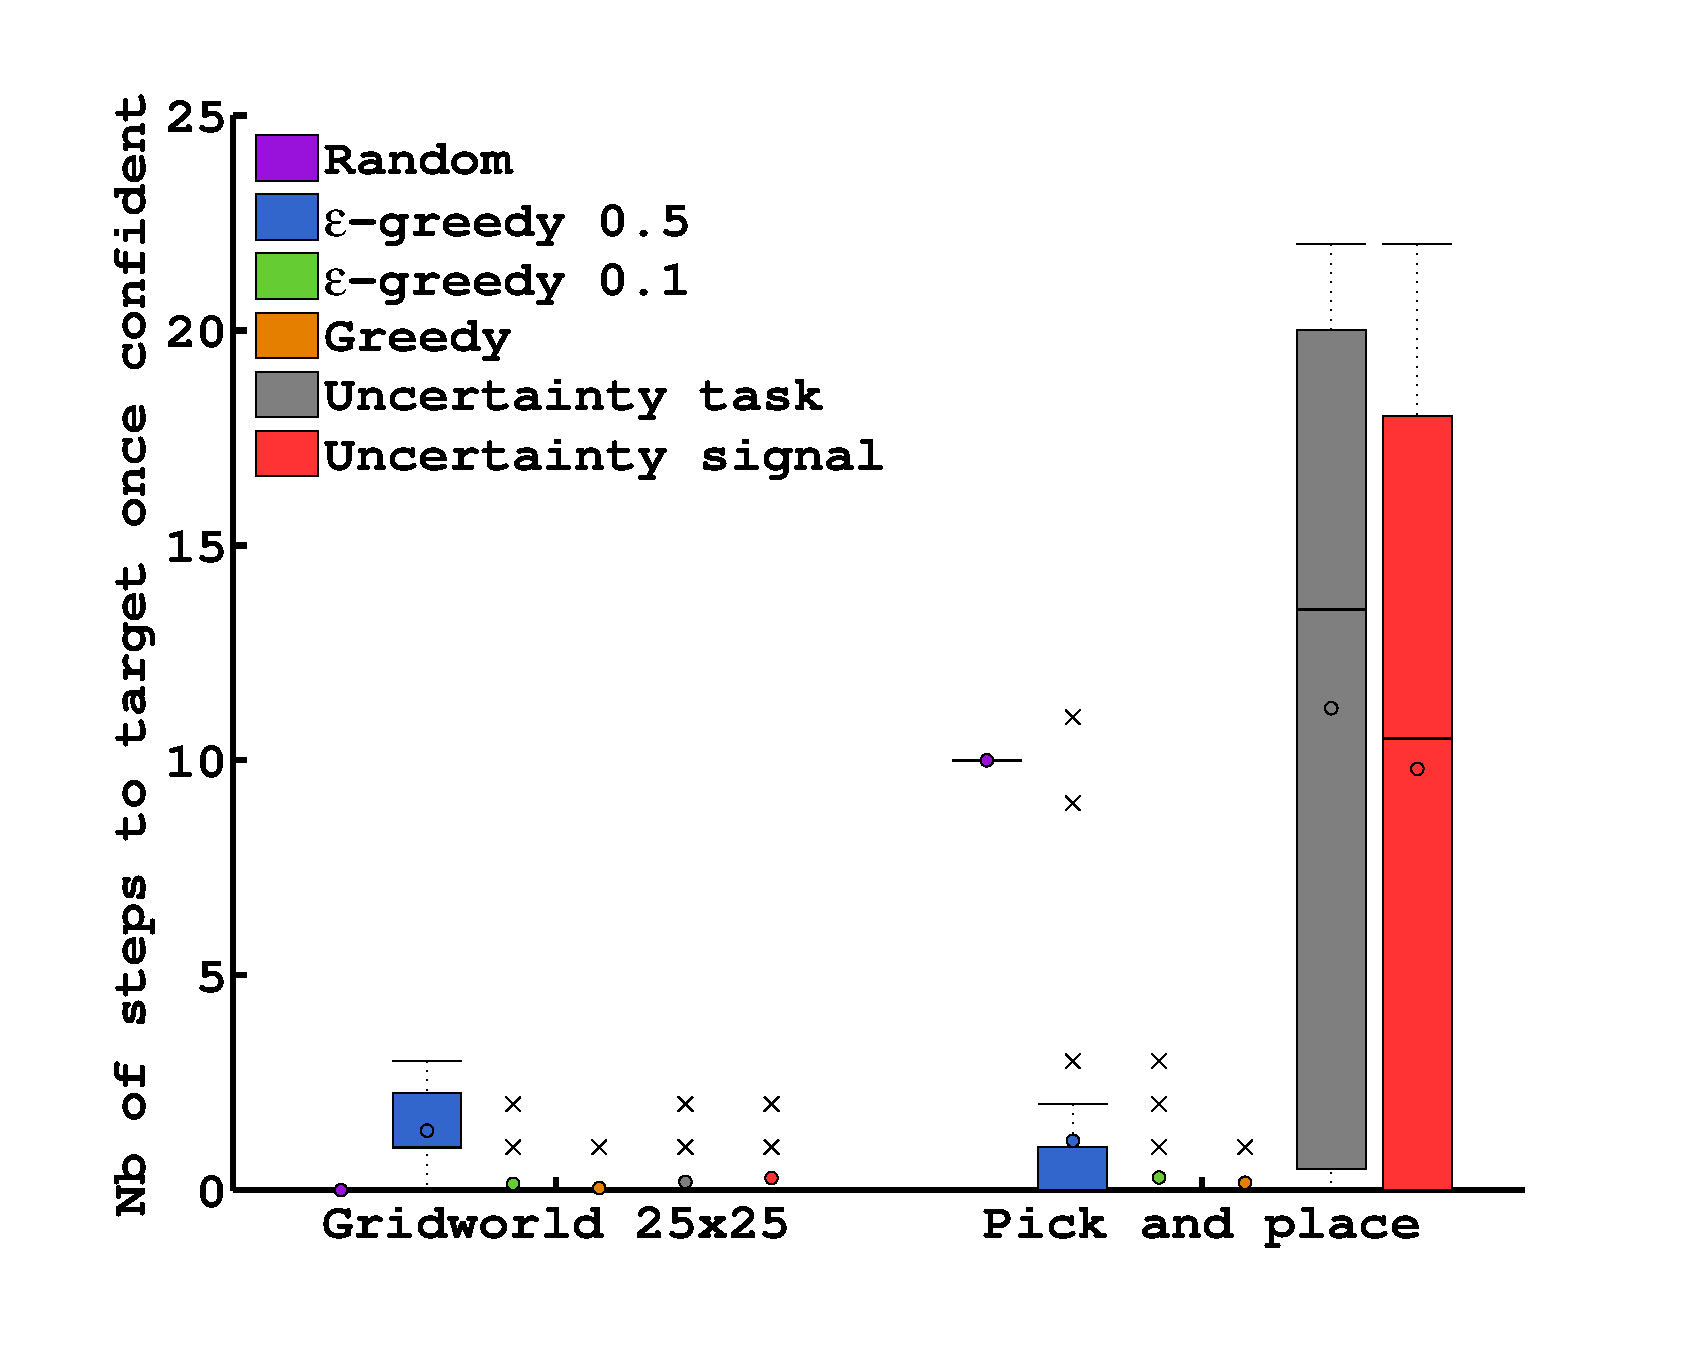
\includegraphics[width=\plotsize\columnwidth]{\imgpath/world_properties/difftargetconfidence.eps}
\caption{Number of action needed to reach the first target when the agent reach confidence level for this target.}
\label{fig:wordlpropertiestargetdist}
\end{figure} 


\begin{table}[!ht]
\centering
\rowcolors{2}{gray!25}{white}
\begin{tabular}{c c c c}
    Planning method & Gridworld &  Pick and place \\ \hline
    Random & 0 & 1 \\ 
    $\epsilon$-greedy 0.5 & 13 & 27 \\
    $\epsilon$-greedy 0.1 & 48 & 48 \\
    Greedy & 43 & 47 \\
    Uncertainty task & 42 & 48 \\
    Uncertainty signal & 50 & 50 \\
\end{tabular}
\caption{Number of experiments that reached at least one target in 100 steps.}
\label{tab:}
\end{table}


